\documentclass[12pt, a4paper]{article}

% PRÉAMBULE -------------------------------------------------------------------

\usepackage[french]{babel}
\usepackage{textcomp}
\usepackage{amsmath}
\usepackage{amsfonts}
\usepackage{graphicx}
\usepackage[T1]{fontenc}
\usepackage{listings}
\usepackage{color}
\usepackage[utf8]{inputenc}

\definecolor{codegreen}{rgb}{0,0.6,0}
\definecolor{codegray}{rgb}{0.5,0.5,0.5}
\definecolor{codepurple}{rgb}{0.58,0,0.82}
\definecolor{backcolour}{rgb}{0.95,0.95,0.92}

\lstdefinestyle{mystyle}{
    backgroundcolor=\color{backcolour},
    commentstyle=\color{codegreen},
    keywordstyle=\color{magenta},
    numberstyle=\tiny\color{codegray},
    stringstyle=\color{codepurple},
    basicstyle=\scriptsize,
    breakatwhitespace=true,
    breaklines=true,
    captionpos=b,
    keepspaces=true,
    numbers=left,
    numbersep=5pt,
    showspaces=false,
    showstringspaces=false,
    showtabs=false,
    tabsize=2
}

\lstset{
     literate=%
        {à}{{\`a}}1
        {é}{{\'e}}1
        {è}{{\`e}}1
        {ê}{{\^e}}1
        {ù}{{\`u}}1
        {À}{{\`A}}1
        {É}{{\'E}}1
        {È}{{\`E}}1
        {Ù}{{\`U}}1
}

\lstset{style=mystyle}

\newcommand{\annexe}[1]{
    \begin{flushright}
    \small{\emph{#1}}
    \end{flushright}
}

\title{Projet ISN - Terminale S - Démineur}

\author{BOURGET Alexis, LE TERTE Dorian, MIGADEL Kevin - TS1}

\date{Année Scolaire 2015-2016}

% --------------------------------------------------------------- FIN PRÉAMBULE

\begin{document}

\pagenumbering{gobble} % Pas de numéro sur la première page
\maketitle
\centerline{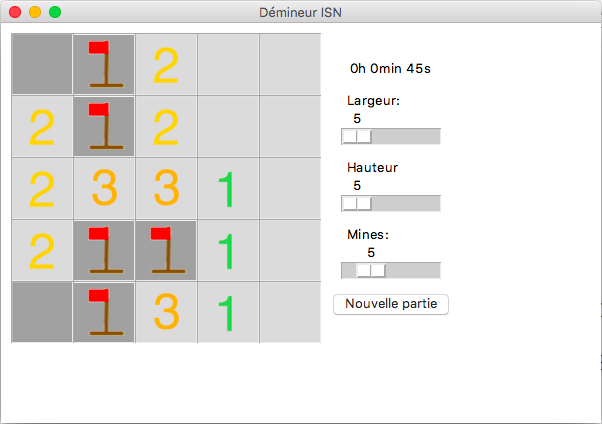
\includegraphics[scale=0.5]{presentation_projet.png}}
\newpage
\pagenumbering{roman}
\tableofcontents % Génère la table des matières ((sub)sub)sections
\lstlistoflistings
\newpage
\pagenumbering{arabic} % Passe la numérotation des pages en chiffres arabes

% CONTENU ---------------------------------------------------------------------

% SECTION ---------------------------------------------------------------------
\section{Présentation du projet}

\paragraph{Pourquoi ce projet ?}
Nous avons choisi de créer un démineur car, malgré son apparente simplicité,
ce n'est pas un jeu simple. En effet, il faut créer un générateur de terrain
qui soit le plus aléatoire et le plus rapide possible et qui place correctement
les numéros sur les cases. De plus, l'interface graphique associée doit
répondre à plusieurs évènements (clic sur le terrain ou non, clic gauche ou
droit, clic sur une case découverte ou non, ...).

\paragraph{Ce qui existait déjà:}
Nous avons effectué des recherches pour nous informer sur les solutions
existantes sur le Web (sur Github notamment). Nous avons trouvé au final assez
peu de ressources: nous cherchions principalement des sources graphiques pour
les éléments du jeu mais n'en n'avons pas trouvées et les avons faites à la
main. \\
Pour ce qui est du code, nous avons éviter de regarder ce qui avait déjà été
fait pour ne pas copier, surtout quand il s'agissait de code Python.

\paragraph{Ce que nous avons obtenu des recherches sur le Web:}
J'ai lu beaucoup de code sur Github, que ce soit en C, C++, C\# ou Java sur
Github afin d'avoir une idée de la logique derrière un démineur. Ce qui est
ressorti est qu'il existe tellement d'approches différentes qu'il y en a
quasiment une par projet. \\
Les codes lus étaient soit en anglais soit en français. J'ai trouvé des
exemples basés sur la programmation orienté objet, d'autres sur un paradigme
fonctionnel et enfin certains utilisaient des boucles évènementielles.

\paragraph{Principe:}
Notre démineur est classique: il faut révéler toutes les cases non-minées du
terrain sans toucher une case minée au passage. Pour cela, les cases sont
numérotées en fonction du nombre de mines dans leur entourage direct.
Le joueur peut placer/supprimer des drapeaux à sa guise.

% ----------------------------------------------------------------- FIN SECTION

\newpage

% SECTION ---------------------------------------------------------------------
\section{Les idées et objectifs du projet}

% SUBsection ------------------------------------------------------------------
\subsection{Cahier des charges du projet}

\paragraph{}
Pour réaliser ce projet au mieux possible avec nos capacités nous avons choisi
de limiter la charge de travail. Ainsi ils existent de nombreuses améliorations
possibles pour notre démineur. Voici toutefois les idées qui nous ont servies
de base de départ: \\

\begin{itemize}
\item Génération d'un terrain miné aléatoire, de la taille demandée
(avec un taille minimum et maximum),
\item Adapter la taille des cases aux dimensions du terrains,
\item Pouvoir relancer une partie sans relancer l'application,
\item Pouvoir placer/enlever des drapeaux sur les cases non-découvertes,
\item Avoir un chronomètre mesurant la durée de la partie,
\item Placer une mine de couleur différente des autres pour signaler celle qui,
le cas échéant, a fait perdre la partie,
\item Afficher un message de fin de partie,
\item Pouvoir propager la révélation des cases si l'on clique sur une case sans
mines aux alentours ou pour révéler le terrain en fin de partie
\end{itemize}

% -------------------------------------------------------------- fin SUBsection

% SUBsection ------------------------------------------------------------------
\subsection{Moyens de réalisation du projet}

\paragraph{Choix du langage:}
Nous avons choisi d'utiliser le langage \emph{Python} en version 3.5. Ce choix
a été motivé par plusieurs raisons. La première raison était que nous avions
tous étudié ce langage au cours de l'année et le connaissions donc un minimum.
La seconde raison est la communauté Python, qu'elle soit française ou anglaise,
qui est très développée et active et donc plus à même de nous aider en cas
de problème important. La dernière raison était plus spécifique à notre groupe,
puisqu'elle vient du fait que j'ai déjà beaucoup codé en Python, que ce soit
pour des programmes graphiques ou en ligne de commande. \\
Nous avons utilisé uniquement la bibliothèque \emph{tkinter} pour notre projet,
afin de le rendre jouable sur un maximum de systèmes d'exploitations d'un coup.

\paragraph{Choix du `type' de code:}
Nous avons choisi d'écrire du code sous forme de fonctions et en partant sur
une gestion évènementielle du démineur. Cela nous a évité de manipuler les
classes, trop compliquées pour nous. Nous avons toutefois fait une exception
pour le chronomètre car la solution utilisant une classe était à la fois la
plus simple et la plus élégante.

% -------------------------------------------------------------- fin SUBsection
% ----------------------------------------------------------------- FIN SECTION

\newpage

% SECTION ---------------------------------------------------------------------
\section{Organisation du travail en groupe}

% SUBsection ------------------------------------------------------------------
\subsection{Répartition des tâches}

\paragraph{}
Nous avons réparti les différentes tâches au sein du groupe de la manière
suivante, en tenant compte de nos niveaux respectifs et de nos envies. \\
Par exemple, j'avais envie de m'occuper de la génération du terrain car cela
me semblait un défi intéressant, je l'ai donc choisi quand personne n'a
protesté contre.

\begin{itemize}
\item Alexis: \emph{Génération du terrain + interface},
\item Dorian: \emph{Gestion du temps},
\item Kévin: \emph{Gestion des actions pour rejouer et pour perdre}.
\end{itemize}

% -------------------------------------------------------------- fin SUBsection

% SUBsection ------------------------------------------------------------------
\subsection{Moyens de collaboration}

\paragraph{Skype:}
Nous avons utilisé Skype pour nous parler régulièrement et échanger nos progrès
sur le code du démineur. Nous avons organisé plusieurs soirées/après-midi où
nous étions deux ou trois à discuter sur comment coder une idée particulière
afin qu'elle s'intègre dans le projet et s'assurer qu'elle fonctionne ailleurs
que sur l'ordinateur du codeur originel.

\paragraph{Github:}
Nous avons aussi utilisé Github car j'en avais déjà l'usage pour d'autres
projets et que son utilisation basique est assez simple. Nous avons utilisé
deux branches: une branche \emph{dev} pour nous échanger les fichiers sans
qu'ils soient forcément compatibles et la branche de base \emph{master} pour
le programme fonctionnel. Cela nous assurait de plus une sauvegarde sure des
fichiers de code et des éléments graphiques.

\paragraph{Documentation:}
J'ai beaucoup insisté pour que la documentation et les commentaires soient
aussi complets et détaillés que possibles. Cela nous a permis de partir du
travail d'un autre sans avoir à recomprendre sa manière de réfléchir en lisant
du code et nous rendait capable de travailler de notre côté sans avoir besoin
d'aide à chaque utilisation d'un code écrit par un autre membre du projet. \\
Ainsi les signatures des fonctions devaient être aussi complètes que possible,
avec la valeur de retour signalée (grâce aux possibilités de Python 3.5).
\annexe{Documentation: voir Annexes - Listing 1}

% -------------------------------------------------------------- fin SUBsection
% ----------------------------------------------------------------- FIN SECTION

\newpage

% SECTION ---------------------------------------------------------------------
\section{Réalisation}

\paragraph{}
Dans cette partie, je vais présenter ce que j'ai fait et les difficultés
rencontrées durant la réalisation des tâches qui m'étaient attribuées.

% SUBsection ------------------------------------------------------------------
\subsection{Génération du terrain}

\paragraph{Objectif:}
Je devais créer un ensemble de fonctions capables de faire les actions
suivantes:

\begin{itemize}
\item Générer un terrain de largeur et la hauteur demandées,
\item Placer les mines sur ce terrain,
\item Placer les chiffres dans les cases entourant les mines.
\end{itemize}

\paragraph{Réalisation:}
J'ai donc créé quatre fonctions pour faire cela. \\
• La première fonction, $\emph{entourage\_case}$, permet de compter les mines
autour d'une case. \\
• $\emph{place\_mines}$ place le nombre de mines demandées sur un terrain vide,
de façon aléatoire. \\
• $\emph{place\_nb\_mines}$ place le nombre de mines adjacentes dans chaque
case. Cette fonction utilise la première, présentée plus haut. \\
• $\emph{genere\_terrain}$ fait usage des deux fonctions précédentes pour
créer un terrain à partir des choix de l'utilisateur quant à la largeur, la
hauteur et le nombre de mines. \\
J'ai aussi créé une fonction $\emph{affiche\_terrain}$ pour pouvoir tester le
bon fonctionnement des fonctions précédentes au cours du développement.

\paragraph{Résultats:}
Voici les résultats que j'obtiens lorsque j'utilise $\emph{affiche\_terrain}$
pour générer divers terrains.

\begin{center}
$\underbrace{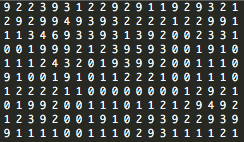
\includegraphics[scale=0.90]{terrains_exemples.png}}_{\text{Un
terrain de 20x10 avec 40 mines.}}$
\end{center}

\annexe{affiche\_terrain: voir Annexes - Listing 2 \\
entourage\_case: voir Annexes - Listing 5}

\paragraph{Problèmes rencontrés:}
J'ai eu à corriger des problèmes d'indexation lorsque de je codais la fonction
qui compte les mines dans l'entourage d'une case. En effet, avec les cases en
bordure il a fallu prendre en compte le fait que pour Python, faire un $-1$
comme index revient à partir de la fin de liste, ce qui ajoutait parfois une
mine qui n'aurait pas due être comptée pour cette case. \\
Un autre problème a été le placement aléatoires des mines. Avec la première
version de ma fonction, les mines étaient toutes alignées sur une colonne à
cause d'une erreur de réfèrencement. Après m'être renseigné sur le problème,
il a été assez facile à corriger, il venait de la façon dont la double liste
représentant le terrain était générée.

\annexe{Problèmes d'index: voir Annexes - Listings 3 et 4}

% -------------------------------------------------------------- fin SUBsection

% SUBsection ------------------------------------------------------------------
\subsection{Interface du démineur}

\paragraph{Objectif:}
L'interface du démineur devait permettre les actions et montrer les
informations suivantes:

\begin{itemize}
\item Placer le terrain jouable (pouvoir placer et retirer des drapeaux,
révéler les cases sans drapeaux, placer le sprite correspondant à la case),
\item Créer les éléments graphiques pour le jeu (puisque nous n'avons rien
trouvé à nos goûts),
\item Permettre de rejouer une partie,
\item Permettre de sélectionner la largeur, la hauteur et le nombre de mines,
\item Afficher la durée de la partie.
\end{itemize}

\paragraph{Réalisation:}
J'ai utilisé \emph{tkinter} pour réaliser l'interface. Cela permet une
portabilité plus importante qu'avec d'autres bibliothèques, facilite
l'utilisation du programmme et simplifie son partage. \\
Pour le terrain de jeu, j'ai utilisé un objet \emph{Canvas}. Pour les réglages
du jeu, j'ai utilisé des \emph{Scale}, \emph{Label} et \emph{Button} à
l'intérieur d'une \emph{Frame}.

\paragraph{Création du plateau de jeu:}
Le plateau de jeu est créé par la fonction \emph{canvas\_plateau(racine: tk.Tk,
largeur: int, hauteur: int, col=0, lig=0)}. Elle commence par nettoyer tout
ce qui a pu être référencé dans les variables importantes. Ainsi l'ancien
plateau est détruit (s'il existe, sinon rien ne se passe) et les variables
référençant les cases sont remises à zéro. Les images du jeu sont alors mises
à jour à leur tour pour être adaptée à la taille du nouveau plateau, puis le
nouveau plateau est initialisé. Enfin les cases sont dessinées une par une
pour remplir le plateau et dans le même temps elles sont référencées de deux
manières: par leur position et par leur \emph{ID} de \emph{Label} que
\emph{tkinter} leur fournit à leur création.
\annexe{canvas\_plateau: voir Annexes - Listing 6}

\paragraph{Résultats:}
À chaque lancement de l'application, un plateau de 5x5 avec 5 mines est généré,
permettant de jouer une partie rapide directement. \\

\centerline{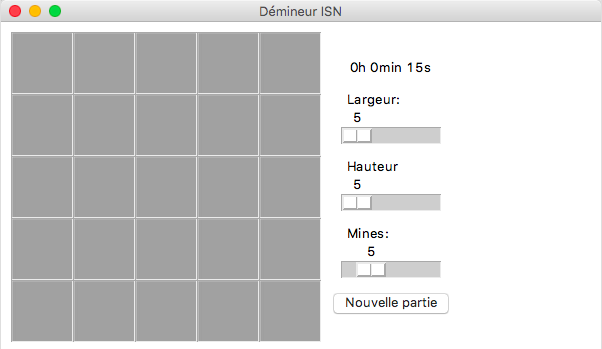
\includegraphics[scale=0.4]{interface_exemple.png}}

\paragraph{Problèmes rencontrés:}
Le premier gros problème que j'ai rencontré a été un problème avec le
\emph{Garbage Collector} de Python, qui supprimait les images quand je tentais
de les référencer. J'ai mis du temps à le comprendre car le code que j'avais
à l'origine s'éxecutait sans problème jusqu'au moment où je cliquais sur une
case, moment où la demande d'accès à une image non référencée faisait planter
le programme. \\
Le problème a été réglé assez rapidement une fois que j'ai cherché sur le Web
mais le temps que j'ai passé à lire la documentation et le code de
\emph{tkinter} n'a absolument pas aidé. \\
La propagation de la révélation des cases a été le second problème important de
l'interface, en présentant deux problèmes en un. Tout d'abord, je n'avais à ce
moment aucun moyen d'accéder aux références des cases via leur position, j'ai
donc dû me résoudre à créer une variable supplémentaire, \emph{cases\_pos}, qui
est un dictionnaire de la forme \emph{\{(int, int): tk.Label\}} et qui
référence les \emph{ID} des cases en fonction de leurs positions en
\emph{(x, y)}. Le second problème était un problème de récursion. En effet,
la fonction \emph{maj\_revele\_case(x: int, y: int)}, dans sa première version,
impliquait un grand nombre de boucles inutiles et posait son return trop tard,
amenant une erreur de récursion trop importante car elle ne vérifiait pas assez
tôt si la case avait été vue auparavant, causant une boucle infinie en
repassant sans arrêt sur les mêmes cases.
\annexe{Problème du Garbage Collector: voir Annexes - Listings 7 et 8 \\
maj\_revele\_case: Listing 9}

% -------------------------------------------------------------- fin SUBsection
% ----------------------------------------------------------------- FIN SECTION

\newpage

% SECTION ---------------------------------------------------------------------
\section{Bilan du projet}

% SUBsection ------------------------------------------------------------------
\subsection{Ce qu'il m'a apporté}

\paragraph{}
Premièrement, je pense que ce que j'ai le plus appris avec ce projet, c'est à
travailler en groupe sur du code. J'utilise souvent Github, mais presque
uniquement pour des projets personnels, afin de me donner un moyen de suivi de
l'évolution et de faciliter le partage si je veux le passer à quelqu'un. \\
J'ai aussi pas mal appris sur la bibliothèque standard de Python (je pense
notamment à la fonction \emph{after} utilisée par Dorian pour le chronomètre)
et sur le module \emph{tkinter}. \\
Je me suis beaucoup amusé avec la récursion, c'était très intéressant de
travailler avec plutôt qu'avec des boucles \emph{while} ou \emph{for}. \\
Enfin, la gestion de modules s'appelant entre eux, les espaces de noms leur
étant attribués et tout le travail pour faire une documentation aussi claire
et complète que possible ont été très formateurs dans leurs domaines.

% -------------------------------------------------------------- fin SUBsection

% SUBsection ------------------------------------------------------------------
\subsection{Ce que nous pourrions améliorer}

\paragraph{Les scores}
Nous avons pensé durant le projet à ajouter des scores avec sauvergarde de ces
derniers pour permettre aux joueurs de se comparer à eux mêmes ou entre eux
mais nous n'avons pas pris le temps de plus réfléchir à l'idée et ne sommes pas
allés plus loin. \\
Nous avions aussi envisagé d'ajouter du son lors des clics sur le plateau, mais
là non plus nous ne sommes pas allés plus loin, principalement par manque de
fichiers de son que nous n'avions pas les moyens d'enregister correctement. \\

% -------------------------------------------------------------- fin SUBsection
% ----------------------------------------------------------------- FIN SECTION

\newpage

% SECTION ---------------------------------------------------------------------
\section*{Annexes: Code}

\paragraph{}
\begin{lstlisting}[language=Python, caption=Exemple de documentation]
def genere_terrain(largeur: int, hauteur: int, nb_mines: int) -> (list, tuple):
    """Génère un terrain comportant nb_mines dans un jeu de largeur * hauteur.

Arguments:
 - largeur          - int - largeur en case du terrain,
 - hauteur          - int - hauteur en case du terrain,
 - nb_mines         - int - le nombre de mines à placer dans le terrain.

Retourne:
 - terrain          - list - le terrain miné avec ses entourages calculés,
 - pos_mines        - tuple - les positions des mines."""

    # On génère un terrain vide
    terrain = [[CASE] * largeur for _ in range(hauteur)]

    # On y place les mines
    terrain = place_mines(terrain, nb_mines)

    # On calcule l'entourage et on récupère le terrain et la position des mines
    terrain, pos_mines = place_nb_mines(terrain)

    return terrain, pos_mines
\end{lstlisting}

\paragraph{}
\begin{lstlisting}[language=Python, caption=Exemple des tests réalisés (ici le
fichier \emph{terrain.py})]
if __name__ == '__main__':
    affiche_terrain(genere_terrain(20, 10, 40)[0])
    affiche_terrain(genere_terrain(8, 8, 20)[0])
\end{lstlisting}

\paragraph{Problèmes d'index - Fonction \emph{entourage\_case}}:
\begin{lstlisting}[language=Python, caption=Premier problème d'index]
try:
    if self.terrain[y-1][x-1]:
        self.terrain[y][x] += 1
except IndexError:
    pass
\end{lstlisting}

\begin{lstlisting}[language=Python, caption=Second problème d'index]
try:
    if self.terrain[abs(y-1)][abs(x-1)]:
        self.terrain[y][x] += 1
except IndexError:
    pass
\end{lstlisting}

\newpage

\begin{lstlisting}[language=Python, caption=Fonction \emph{entourage\_case}
finale]
def entourage_case(terrain: list, x: int, y: int) -> (list):
    """Retourne l'entourage d'une case donnée dans un terrain donné.

Arguments:
 - terrain      - list - le terrain dans lequel agir,
 - x            - int - la coordonnée x de la case dont on veut l'entourage,
 - y            - int - la coordonnée y de la case dont on veut l'entourage.

Retourne:
 - entourage    - list - la liste contenant l'entourage de la case."""

    # Si y-1 ou x-1 = -1, on risque d'accéder au mauvais élément de terrain
    # lors de la vérification de l'entourage de la case donc on le place
    # volontairement en dehors des possibilités d'accès afin de lever une
    # erreur et d'ajouter une CASE au lieu de recompter une MINE lors de
    # la vérification
    y_moins = y - 1 if y - 1 >= 0 else len(terrain)
    x_moins = x - 1 if x - 1 >= 0 else len(terrain[0])

    # L'entourage de la case vérifiée
    entourage = []

    # Haut, à gauche
    try: entourage.append(terrain[y_moins][x_moins])
    except IndexError: entourage.append(CASE)

    # Haut, au milieu
    try: entourage.append(terrain[y_moins][x])
    except IndexError: entourage.append(CASE)

    # Haut, à droite
    try: entourage.append(terrain[y_moins][x+1])
    except IndexError: entourage.append(CASE)

    # Milieu, à droite
    try: entourage.append(terrain[y][x+1])
    except IndexError: entourage.append(CASE)

    # Bas, à droite
    try: entourage.append(terrain[y+1][x+1])
    except IndexError: entourage.append(CASE)

    # Bas, au milieu
    try: entourage.append(terrain[y+1][x])
    except IndexError: entourage.append(CASE)

    # Bas, à gauche
    try: entourage.append(terrain[y+1][x_moins])
    except IndexError: entourage.append(CASE)

    # Milieu, à gauche
    try: entourage.append(terrain[y][x_moins])
    except IndexError: entourage.append(CASE)

    return entourage
\end{lstlisting}

\newpage

\begin{lstlisting}[language=Python, caption=Fonction \emph{canvas\_plateau}]
def canvas_plateau(racine: tk.Tk,
                   largeur: int, hauteur: int,
                   col=0, lig=0) -> (None):
    """Dessine le plateau de base du jeu, avant que l'utilisateur ne commence \
à jouer.

Argument:
 - racine       - tk.Tk - la fenêtre dans laquelle dessiner le plateau,
 - largeur      - int - largeur en case du terrain,
 - hauteur      - int - hauteur en case du terrain,
 - col=0        - int - la colonne de la racine où sera placé le plateau,
 - lig=0        - int - la ligne de la racine où sera placé le plateau.

Modifie:
 - cv_plateau   - tk.Canvas - le plateau du jeu."""

    global cv_plateau, cases_taille, cases, cases_pos

    # On nettoie le plateau précédent, on remet à zéro les variables en ayant
    # besoin
    cv_plateau.destroy()
    cases = {}
    cases_pos = {}

    # On met à jour les images
    maj_taille_cases(largeur, hauteur)
    maj_images(cv_plateau, cases_taille)

    # Initialise le nouveau plateau
    cv_plateau = tk.Canvas(racine,
                           width=largeur * cases_taille,
                           height=hauteur * cases_taille)
    # Place le plateau
    cv_plateau.grid(column=col, row=lig, padx=10, pady=10)

    # Dessine les cases du jeu
    for y in range(hauteur):
        for x in range(largeur):
            # Récupère la référence en dessinant la case
            case = label_case(cv_plateau, x, y)
            # Associe la référence de la case à ses coordonnées (x, y)
            cases[case] = (x, y)
            # Associe les coordonnées (x, y) à la référence de la case
            cases_pos[(x, y)] = case
\end{lstlisting}

\newpage

\paragraph{Problèmes du \emph{Garbage Collector}}:

\paragraph{}
\begin{lstlisting}[language=Python, caption=Version 1 de \emph{cases\_img}]
cases_img = {
    0:        tk.PhotoImage(file='%scase_0.gif' % chemin),
    1:        tk.PhotoImage(file='%scase_1.gif' % chemin),
    2:        tk.PhotoImage(file='%scase_2.gif' % chemin),
    3:        tk.PhotoImage(file='%scase_3.gif' % chemin),
    4:        tk.PhotoImage(file='%scase_4.gif' % chemin),
    5:        tk.PhotoImage(file='%scase_5.gif' % chemin),
    6:        tk.PhotoImage(file='%scase_6.gif' % chemin),
    7:        tk.PhotoImage(file='%scase_7.gif' % chemin),
    8:        tk.PhotoImage(file='%scase_8.gif' % chemin),
    BASE:     tk.PhotoImage(file='%sbase.gif' % chemin),
    DRAPEAU:  tk.PhotoImage(file='%sdrapeau.gif' % chemin),
    MINE:     tk.PhotoImage(file='%smine.gif' % chemin),
    PERDU:    tk.PhotoImage(file='%sperdu.gif' % chemin)
}
\end{lstlisting}

\paragraph{}
\begin{lstlisting}[language=Python, caption=Version finale de \emph{cases\_img}]
cases_img = {
    0:        tk.PhotoImage(master=racine, file='%scase_0.gif' % chemin),
    1:        tk.PhotoImage(master=racine, file='%scase_1.gif' % chemin),
    2:        tk.PhotoImage(master=racine, file='%scase_2.gif' % chemin),
    3:        tk.PhotoImage(master=racine, file='%scase_3.gif' % chemin),
    4:        tk.PhotoImage(master=racine, file='%scase_4.gif' % chemin),
    5:        tk.PhotoImage(master=racine, file='%scase_5.gif' % chemin),
    6:        tk.PhotoImage(master=racine, file='%scase_6.gif' % chemin),
    7:        tk.PhotoImage(master=racine, file='%scase_7.gif' % chemin),
    8:        tk.PhotoImage(master=racine, file='%scase_8.gif' % chemin),
    BASE:     tk.PhotoImage(master=racine, file='%sbase.gif' % chemin),
    DRAPEAU:  tk.PhotoImage(master=racine, file='%sdrapeau.gif' % chemin),
    MINE:     tk.PhotoImage(master=racine, file='%smine.gif' % chemin),
    PERDU:    tk.PhotoImage(master=racine, file='%sperdu.gif' % chemin)
}
\end{lstlisting}

\paragraph{Note}
Les variables notées en majuscules, à l'instar de \emph{BASE}, sont des
constantes issues du fichier \emph{constantes.py}, qui ne sert à rien d'autre
qu'à les enregistrer.

\newpage

\begin{lstlisting}[language=Python, caption=Fonction \emph{maj\_revele\_case}]
def maj_revele_case(x: int, y: int) -> (None):

    global cases, cases_pos, cases_img

    # On récupère la valeur de la case et on continue dans la fonction
    # uniquement si la case n'a pas déjà été révélé
    try: valeur_case = joueur.terrain[y][x]
    except IndexError: return
    finally:
        if (x, y) in joueur.cases_vues:
            return

    # On récupère la case sous sa forme de tk.Label
    case = cases_pos[(x, y)]

    # Si la case est un chiffre basique, on l'affiche
    if 0 < valeur_case < 9:
        joueur.cases_vues.append((x, y))
        case['image'] = cases_img[valeur_case]
    # Si la case vaut zéro, on révèle l'entourage
    elif valeur_case == 0:
        joueur.cases_vues.append((x, y))
        case['image'] = cases_img[valeur_case]

        # Pour éviter les indices négatifs et les problèmes qui vont avec,
        # on provoque une IndexError dans les appels suivants
        y_moins = y - 1 if y - 1 >= 0 else len(joueur.terrain)
        x_moins = x - 1 if x - 1 >= 0 else len(joueur.terrain[0])

        # On teste les cases autour, pour les révéler ou propager la révélation
        # si elles sont de valeur 0
        # Haut, à gauche
        maj_revele_case(x_moins, y_moins)
        # Haut, au milieu
        maj_revele_case(x, y_moins)
        # Haut, à droite
        maj_revele_case(x+1, y_moins)
        # Milieu, à droite
        maj_revele_case(x+1, y)
        # Bas, à droite
        maj_revele_case(x+1, y+1)
        # Bas, au milieu
        maj_revele_case(x, y+1)
        # Bas, à gauche
        maj_revele_case(x_moins, y+1)
        # Milieu, à gauche
        maj_revele_case(x_moins, y)
    # Si la case n'était pas chiffrée (une mine donc), on la révèle
    else:
        joueur.cases_vues.append((x, y))
        # Affiche la mine de couleur rouge si c'est celle qui fait perdre la
        # partie, sinon la mine noire
        if not ordi.fini: case['image'] = cases_img[PERDU]
        else: case['image'] = cases_img[MINE]

    ordi.nb_cases_vues += 1
    ordi.verif_etat_partie(valeur_case)
\end{lstlisting}

% ----------------------------------------------------------------- FIN SECTION

% ----------------------------------------------------------------- FIN CONTENU
\end{document}
